\documentclass[1p]{elsarticle_modified}
%\bibliographystyle{elsarticle-num}

%\usepackage[colorlinks]{hyperref}
%\usepackage{abbrmath_seonhwa} %\Abb, \Ascr, \Acal ,\Abf, \Afrak
\usepackage{amsfonts}
\usepackage{amssymb}
\usepackage{amsmath}
\usepackage{amsthm}
\usepackage{scalefnt}
\usepackage{amsbsy}
\usepackage{kotex}
\usepackage{caption}
\usepackage{subfig}
\usepackage{color}
\usepackage{graphicx}
\usepackage{xcolor} %% white, black, red, green, blue, cyan, magenta, yellow
\usepackage{float}
\usepackage{setspace}
\usepackage{hyperref}

\usepackage{tikz}
\usetikzlibrary{arrows}

\usepackage{multirow}
\usepackage{array} % fixed length table
\usepackage{hhline}

%%%%%%%%%%%%%%%%%%%%%
\makeatletter
\renewcommand*\env@matrix[1][\arraystretch]{%
	\edef\arraystretch{#1}%
	\hskip -\arraycolsep
	\let\@ifnextchar\new@ifnextchar
	\array{*\c@MaxMatrixCols c}}
\makeatother %https://tex.stackexchange.com/questions/14071/how-can-i-increase-the-line-spacing-in-a-matrix
%%%%%%%%%%%%%%%

\usepackage[normalem]{ulem}

\newcommand{\msout}[1]{\ifmmode\text{\sout{\ensuremath{#1}}}\else\sout{#1}\fi}
%SOURCE: \msout is \stkout macro in https://tex.stackexchange.com/questions/20609/strikeout-in-math-mode

\newcommand{\cancel}[1]{
	\ifmmode
	{\color{red}\msout{#1}}
	\else
	{\color{red}\sout{#1}}
	\fi
}

\newcommand{\add}[1]{
	{\color{blue}\uwave{#1}}
}

\newcommand{\replace}[2]{
	\ifmmode
	{\color{red}\msout{#1}}{\color{blue}\uwave{#2}}
	\else
	{\color{red}\sout{#1}}{\color{blue}\uwave{#2}}
	\fi
}

\newcommand{\Sol}{\mathcal{S}} %segment
\newcommand{\D}{D} %diagram
\newcommand{\A}{\mathcal{A}} %arc


%%%%%%%%%%%%%%%%%%%%%%%%%%%%%5 test

\def\sl{\operatorname{\textup{SL}}(2,\Cbb)}
\def\psl{\operatorname{\textup{PSL}}(2,\Cbb)}
\def\quan{\mkern 1mu \triangleright \mkern 1mu}

\theoremstyle{definition}
\newtheorem{thm}{Theorem}[section]
\newtheorem{prop}[thm]{Proposition}
\newtheorem{lem}[thm]{Lemma}
\newtheorem{ques}[thm]{Question}
\newtheorem{cor}[thm]{Corollary}
\newtheorem{defn}[thm]{Definition}
\newtheorem{exam}[thm]{Example}
\newtheorem{rmk}[thm]{Remark}
\newtheorem{alg}[thm]{Algorithm}

\newcommand{\I}{\sqrt{-1}}
\begin{document}

%\begin{frontmatter}
%
%\title{Boundary parabolic representations of knots up to 8 crossings}
%
%%% Group authors per affiliation:
%\author{Yunhi Cho} 
%\address{Department of Mathematics, University of Seoul, Seoul, Korea}
%\ead{yhcho@uos.ac.kr}
%
%
%\author{Seonhwa Kim} %\fnref{s_kim}}
%\address{Center for Geometry and Physics, Institute for Basic Science, Pohang, 37673, Korea}
%\ead{ryeona17@ibs.re.kr}
%
%\author{Hyuk Kim}
%\address{Department of Mathematical Sciences, Seoul National University, Seoul 08826, Korea}
%\ead{hyukkim@snu.ac.kr}
%
%\author{Seokbeom Yoon}
%\address{Department of Mathematical Sciences, Seoul National University, Seoul, 08826,  Korea}
%\ead{sbyoon15@snu.ac.kr}
%
%\begin{abstract}
%We find all boundary parabolic representation of knots up to 8 crossings.
%
%\end{abstract}
%\begin{keyword}
%    \MSC[2010] 57M25 
%\end{keyword}
%
%\end{frontmatter}

%\linenumbers
%\tableofcontents
%
\newcommand\colored[1]{\textcolor{white}{\rule[-0.35ex]{0.8em}{1.4ex}}\kern-0.8em\color{red} #1}%
%\newcommand\colored[1]{\textcolor{white}{ #1}\kern-2.17ex	\textcolor{white}{ #1}\kern-1.81ex	\textcolor{white}{ #1}\kern-2.15ex\color{red}#1	}

{\Large $\underline{12a_{0982}~(K12a_{0982})}$}

\setlength{\tabcolsep}{10pt}
\renewcommand{\arraystretch}{1.6}
\vspace{1cm}\begin{tabular}{m{100pt}>{\centering\arraybackslash}m{274pt}}
\multirow{5}{120pt}{
	\centering
	\includegraphics[width=112pt]{../../../GIT/diagram.site/Diagrams/png/1783_12a_0982.png}\\
\ \ \ A knot diagram\footnotemark}&
\allowdisplaybreaks
\textbf{Linearized knot diagam} \\
\cline{2-2}
 &
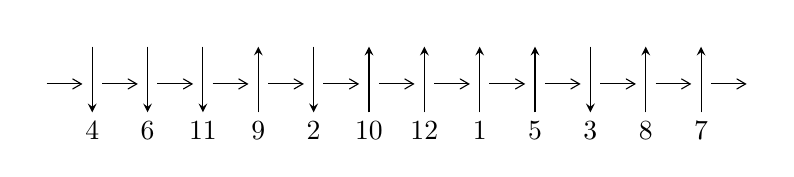
\begin{tikzpicture}[x=20pt, y=17pt]
	% nodes
	\node (C0) at (0, 0) {};
	\node (C1) at (1, 0) {};
	\node (C1U) at (1, +1) {};
	\node (C1D) at (1, -1) {4};

	\node (C2) at (2, 0) {};
	\node (C2U) at (2, +1) {};
	\node (C2D) at (2, -1) {6};

	\node (C3) at (3, 0) {};
	\node (C3U) at (3, +1) {};
	\node (C3D) at (3, -1) {11};

	\node (C4) at (4, 0) {};
	\node (C4U) at (4, +1) {};
	\node (C4D) at (4, -1) {9};

	\node (C5) at (5, 0) {};
	\node (C5U) at (5, +1) {};
	\node (C5D) at (5, -1) {2};

	\node (C6) at (6, 0) {};
	\node (C6U) at (6, +1) {};
	\node (C6D) at (6, -1) {10};

	\node (C7) at (7, 0) {};
	\node (C7U) at (7, +1) {};
	\node (C7D) at (7, -1) {12};

	\node (C8) at (8, 0) {};
	\node (C8U) at (8, +1) {};
	\node (C8D) at (8, -1) {1};

	\node (C9) at (9, 0) {};
	\node (C9U) at (9, +1) {};
	\node (C9D) at (9, -1) {5};

	\node (C10) at (10, 0) {};
	\node (C10U) at (10, +1) {};
	\node (C10D) at (10, -1) {3};

	\node (C11) at (11, 0) {};
	\node (C11U) at (11, +1) {};
	\node (C11D) at (11, -1) {8};

	\node (C12) at (12, 0) {};
	\node (C12U) at (12, +1) {};
	\node (C12D) at (12, -1) {7};
	\node (C13) at (13, 0) {};

	% arrows
	\draw[->,>={angle 60}]
	(C0) edge (C1) (C1) edge (C2) (C2) edge (C3) (C3) edge (C4) (C4) edge (C5) (C5) edge (C6) (C6) edge (C7) (C7) edge (C8) (C8) edge (C9) (C9) edge (C10) (C10) edge (C11) (C11) edge (C12) (C12) edge (C13) ;	\draw[->,>=stealth]
	(C1U) edge (C1D) (C2U) edge (C2D) (C3U) edge (C3D) (C4D) edge (C4U) (C5U) edge (C5D) (C6D) edge (C6U) (C7D) edge (C7U) (C8D) edge (C8U) (C9D) edge (C9U) (C10U) edge (C10D) (C11D) edge (C11U) (C12D) edge (C12U) ;
	\end{tikzpicture} \\
\hhline{~~} \\& 
\textbf{Solving Sequence} \\ \cline{2-2} 
 &
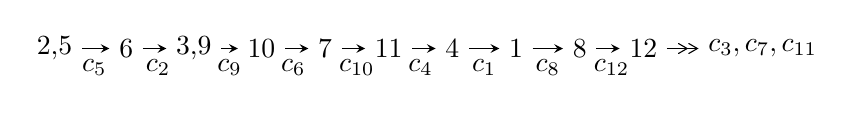
\begin{tikzpicture}[x=23pt, y=7pt]
	% node
	\node (A0) at (-1/8, 0) {2,5};
	\node (A1) at (1, 0) {6};
	\node (A2) at (33/16, 0) {3,9};
	\node (A3) at (25/8, 0) {10};
	\node (A4) at (33/8, 0) {7};
	\node (A5) at (41/8, 0) {11};
	\node (A6) at (49/8, 0) {4};
	\node (A7) at (57/8, 0) {1};
	\node (A8) at (65/8, 0) {8};
	\node (A9) at (73/8, 0) {12};
	\node (C1) at (1/2, -1) {$c_{5}$};
	\node (C2) at (3/2, -1) {$c_{2}$};
	\node (C3) at (21/8, -1) {$c_{9}$};
	\node (C4) at (29/8, -1) {$c_{6}$};
	\node (C5) at (37/8, -1) {$c_{10}$};
	\node (C6) at (45/8, -1) {$c_{4}$};
	\node (C7) at (53/8, -1) {$c_{1}$};
	\node (C8) at (61/8, -1) {$c_{8}$};
	\node (C9) at (69/8, -1) {$c_{12}$};
	\node (A10) at (11, 0) {$c_{3},c_{7},c_{11}$};

	% edge
	\draw[->,>=stealth]	
	(A0) edge (A1) (A1) edge (A2) (A2) edge (A3) (A3) edge (A4) (A4) edge (A5) (A5) edge (A6) (A6) edge (A7) (A7) edge (A8) (A8) edge (A9) ;
	\draw[->>,>={angle 60}]	
	(A9) edge (A10);
\end{tikzpicture} \\ 

\end{tabular} \\

\footnotetext{
The image of knot diagram is generated by the software ``\textbf{Draw programme}" developed by Andrew Bartholomew(\url{http://www.layer8.co.uk/maths/draw/index.htm\#Running-draw}), where we modified some parts for our purpose(\url{https://github.com/CATsTAILs/LinksPainter}).
}\phantom \\ \newline 
\centering \textbf{Ideals for irreducible components\footnotemark of $X_{\text{par}}$} 
 
\begin{align*}
I^u_{1}&=\langle 
396741557 u^{70}-2705520519 u^{69}+\cdots+3439853568 b+8641755965218,\\
\phantom{I^u_{1}}&\phantom{= \langle  }120849802046 u^{70}-453217535127 u^{69}+\cdots+16303759294464 a-3531490614456158,\\
\phantom{I^u_{1}}&\phantom{= \langle  }u^{71}-8 u^{70}+\cdots+300422 u-28438\rangle \\
I^u_{2}&=\langle 
- a^2+b- a,\;a^3+2 a^2+a+1,\;u+1\rangle \\
I^u_{3}&=\langle 
b^6 a^3+3 b^5 a^2+\cdots- a^2+1,\;u+1\rangle \\
\\
I^v_{1}&=\langle 
a,\;b^9-3 b^7- b^6+3 b^5+2 b^4- b^3- b^2+1,\;v-1\rangle \\
I^v_{2}&=\langle 
a,\;b+1,\;v-1\rangle \\
\end{align*}
\raggedright * 4 irreducible components of $\dim_{\mathbb{C}}=0$, with total 84 representations.\\
\raggedright * 1 irreducible components of $\dim_{\mathbb{C}}=1$ \\
\footnotetext{All coefficients of polynomials are rational numbers. But the coefficients are sometimes approximated in decimal forms when there is not enough margin.}
\newpage
\renewcommand{\arraystretch}{1}
\centering \section*{I. $I^u_{1}= \langle 3.97\times10^{8} u^{70}-2.71\times10^{9} u^{69}+\cdots+3.44\times10^{9} b+8.64\times10^{12},\;1.21\times10^{11} u^{70}-4.53\times10^{11} u^{69}+\cdots+1.63\times10^{13} a-3.53\times10^{15},\;u^{71}-8 u^{70}+\cdots+300422 u-28438 \rangle$}
\flushleft \textbf{(i) Arc colorings}\\
\begin{tabular}{m{7pt} m{180pt} m{7pt} m{180pt} }
\flushright $a_{2}=$&$\begin{pmatrix}0\\u\end{pmatrix}$ \\
\flushright $a_{5}=$&$\begin{pmatrix}1\\0\end{pmatrix}$ \\
\flushright $a_{6}=$&$\begin{pmatrix}1\\u^2\end{pmatrix}$ \\
\flushright $a_{3}=$&$\begin{pmatrix}- u\\- u^3+u\end{pmatrix}$ \\
\flushright $a_{9}=$&$\begin{pmatrix}-0.00741239 u^{70}+0.0277983 u^{69}+\cdots-1878.55 u+216.606\\-0.115337 u^{70}+0.786522 u^{69}+\cdots+24797.7 u-2512.25\end{pmatrix}$ \\
\flushright $a_{10}=$&$\begin{pmatrix}-0.122749 u^{70}+0.814320 u^{69}+\cdots+22919.2 u-2295.64\\-0.115337 u^{70}+0.786522 u^{69}+\cdots+24797.7 u-2512.25\end{pmatrix}$ \\
\flushright $a_{7}=$&$\begin{pmatrix}-0.000272721 u^{70}-0.00335184 u^{69}+\cdots-1221.87 u+147.123\\-0.00543439 u^{70}+0.0380903 u^{69}+\cdots+1475.66 u-154.612\end{pmatrix}$ \\
\flushright $a_{11}=$&$\begin{pmatrix}0.0189981 u^{70}-0.0965360 u^{69}+\cdots+527.401 u-91.8508\\0.0592586 u^{70}-0.423571 u^{69}+\cdots-15810.2 u+1629.10\end{pmatrix}$ \\
\flushright $a_{4}=$&$\begin{pmatrix}-0.00520879 u^{70}+0.0363631 u^{69}+\cdots+1412.36 u-149.354\\-0.000436995 u^{70}+0.00302753 u^{69}+\cdots+98.9193 u-9.63599\end{pmatrix}$ \\
\flushright $a_{1}=$&$\begin{pmatrix}-0.00169434 u^{70}+0.0103657 u^{69}+\cdots+9.95932 u+5.55905\\0.00278897 u^{70}-0.0175826 u^{69}+\cdots-319.666 u+29.2856\end{pmatrix}$ \\
\flushright $a_{8}=$&$\begin{pmatrix}-0.0850548 u^{70}+0.573329 u^{69}+\cdots+17746.1 u-1797.14\\0.0303146 u^{70}-0.166206 u^{69}+\cdots+680.125 u-139.988\end{pmatrix}$ \\
\flushright $a_{12}=$&$\begin{pmatrix}0.00146179 u^{70}+0.0124218 u^{69}+\cdots+2863.44 u-314.383\\0.0395988 u^{70}-0.254642 u^{69}+\cdots-5850.13 u+567.179\end{pmatrix}$\\&\end{tabular}
\flushleft \textbf{(ii) Obstruction class $= -1$}\\~\\
\flushleft \textbf{(iii) Cusp Shapes $= -\frac{1064976745}{5159780352} u^{70}+\frac{767202109}{573308928} u^{69}+\cdots+\frac{3030931480757}{95551488} u-\frac{3956494938221}{1289945088}$}\\~\\
\newpage\renewcommand{\arraystretch}{1}
\flushleft \textbf{(iv) u-Polynomials at the component}\newline \\
\begin{tabular}{m{50pt}|m{274pt}}
Crossings & \hspace{64pt}u-Polynomials at each crossing \\
\hline $$\begin{aligned}c_{1}\end{aligned}$$&$\begin{aligned}
&64(64 u^{71}-64 u^{70}+\cdots+8937 u+2889)
\end{aligned}$\\
\hline $$\begin{aligned}c_{2},c_{5}\end{aligned}$$&$\begin{aligned}
&u^{71}-8 u^{70}+\cdots+300422 u-28438
\end{aligned}$\\
\hline $$\begin{aligned}c_{3},c_{10}\end{aligned}$$&$\begin{aligned}
&27(27 u^{71}-54 u^{70}+\cdots-3 u+1)
\end{aligned}$\\
\hline $$\begin{aligned}c_{4},c_{9}\end{aligned}$$&$\begin{aligned}
&27(27 u^{71}+54 u^{70}+\cdots+u+1)
\end{aligned}$\\
\hline $$\begin{aligned}c_{6}\end{aligned}$$&$\begin{aligned}
&64(64 u^{71}-64 u^{70}+\cdots-1629153 u+409509)
\end{aligned}$\\
\hline $$\begin{aligned}c_{7},c_{11},c_{12}\end{aligned}$$&$\begin{aligned}
&u^{71}+4 u^{70}+\cdots-370 u-46
\end{aligned}$\\
\hline $$\begin{aligned}c_{8}\end{aligned}$$&$\begin{aligned}
&u^{71}-4 u^{70}+\cdots+559616 u-400384
\end{aligned}$\\
\hline
\end{tabular}\\~\\
\newpage\renewcommand{\arraystretch}{1}
\flushleft \textbf{(v) Riley Polynomials at the component}\newline \\
\begin{tabular}{m{50pt}|m{274pt}}
Crossings & \hspace{64pt}Riley Polynomials at each crossing \\
\hline $$\begin{aligned}c_{1}\end{aligned}$$&$\begin{aligned}
&4096(4096 y^{71}-61440 y^{70}+\cdots-1.34847\times10^{9} y-8346321)
\end{aligned}$\\
\hline $$\begin{aligned}c_{2},c_{5}\end{aligned}$$&$\begin{aligned}
&y^{71}-48 y^{70}+\cdots+17125572968 y-808719844
\end{aligned}$\\
\hline $$\begin{aligned}c_{3},c_{10}\end{aligned}$$&$\begin{aligned}
&729(729 y^{71}-36450 y^{70}+\cdots+37 y-1)
\end{aligned}$\\
\hline $$\begin{aligned}c_{4},c_{9}\end{aligned}$$&$\begin{aligned}
&729(729 y^{71}-30618 y^{70}+\cdots+21 y-1)
\end{aligned}$\\
\hline $$\begin{aligned}c_{6}\end{aligned}$$&$\begin{aligned}
&4096\\
&\cdot(4096 y^{71}+45056 y^{70}+\cdots-296794641861 y-167697621081)
\end{aligned}$\\
\hline $$\begin{aligned}c_{7},c_{11},c_{12}\end{aligned}$$&$\begin{aligned}
&y^{71}+60 y^{70}+\cdots+31744 y-2116
\end{aligned}$\\
\hline $$\begin{aligned}c_{8}\end{aligned}$$&$\begin{aligned}
&y^{71}-20 y^{70}+\cdots+1087647252480 y-160307347456
\end{aligned}$\\
\hline
\end{tabular}\\~\\
\newpage\flushleft \textbf{(vi) Complex Volumes and Cusp Shapes}
$$\begin{array}{c|c|c}  
\text{Solutions to }I^u_{1}& \I (\text{vol} + \sqrt{-1}CS) & \text{Cusp shape}\\
 \hline 
\begin{aligned}
u &= \phantom{-}0.819521 + 0.520466 I \\
a &= -1.58110 - 0.82078 I \\
b &= \phantom{-}1.007920 - 0.102626 I\end{aligned}
 & \phantom{-}1.42180 - 0.53019 I & \phantom{-}7.50103 + 0. I\phantom{ +0.000000I} \\ \hline\begin{aligned}
u &= \phantom{-}0.819521 - 0.520466 I \\
a &= -1.58110 + 0.82078 I \\
b &= \phantom{-}1.007920 + 0.102626 I\end{aligned}
 & \phantom{-}1.42180 + 0.53019 I & \phantom{-}7.50103 + 0. I\phantom{ +0.000000I} \\ \hline\begin{aligned}
u &= \phantom{-}0.307366 + 0.904911 I \\
a &= -1.51865 - 0.42035 I \\
b &= \phantom{-}1.289990 + 0.173842 I\end{aligned}
 & \phantom{-}3.63707 - 1.17327 I & \phantom{-}6.61182 + 2.79470 I \\ \hline\begin{aligned}
u &= \phantom{-}0.307366 - 0.904911 I \\
a &= -1.51865 + 0.42035 I \\
b &= \phantom{-}1.289990 - 0.173842 I\end{aligned}
 & \phantom{-}3.63707 + 1.17327 I & \phantom{-}6.61182 - 2.79470 I \\ \hline\begin{aligned}
u &= -1.023520 + 0.258526 I \\
a &= \phantom{-}0.981518 + 0.240605 I \\
b &= \phantom{-}0.499246 - 0.339591 I\end{aligned}
 & -5.41474 + 1.54205 I & \phantom{-0.000000 } 0 \\ \hline\begin{aligned}
u &= -1.023520 - 0.258526 I \\
a &= \phantom{-}0.981518 - 0.240605 I \\
b &= \phantom{-}0.499246 + 0.339591 I\end{aligned}
 & -5.41474 - 1.54205 I & \phantom{-0.000000 } 0 \\ \hline\begin{aligned}
u &= \phantom{-}0.238590 + 0.854323 I \\
a &= \phantom{-}1.48171 + 0.51225 I \\
b &= -1.307940 - 0.307987 I\end{aligned}
 & \phantom{-}6.49722 + 2.98352 I & \phantom{-}9.50430 - 2.12816 I \\ \hline\begin{aligned}
u &= \phantom{-}0.238590 - 0.854323 I \\
a &= \phantom{-}1.48171 - 0.51225 I \\
b &= -1.307940 + 0.307987 I\end{aligned}
 & \phantom{-}6.49722 - 2.98352 I & \phantom{-}9.50430 + 2.12816 I \\ \hline\begin{aligned}
u &= -0.855012\phantom{ +0.000000I} \\
a &= -0.981809\phantom{ +0.000000I} \\
b &= -0.440716\phantom{ +0.000000I}\end{aligned}
 & -1.39100\phantom{ +0.000000I} & -8.59610\phantom{ +0.000000I} \\ \hline\begin{aligned}
u &= \phantom{-}0.198592 + 0.831468 I \\
a &= -1.42804 - 0.58646 I \\
b &= \phantom{-}1.306230 + 0.409174 I\end{aligned}
 & \phantom{-}1.79097 + 6.98426 I & \phantom{-}4.65978 - 4.42101 I\\
 \hline 
 \end{array}$$\newpage$$\begin{array}{c|c|c}  
\text{Solutions to }I^u_{1}& \I (\text{vol} + \sqrt{-1}CS) & \text{Cusp shape}\\
 \hline 
\begin{aligned}
u &= \phantom{-}0.198592 - 0.831468 I \\
a &= -1.42804 + 0.58646 I \\
b &= \phantom{-}1.306230 - 0.409174 I\end{aligned}
 & \phantom{-}1.79097 - 6.98426 I & \phantom{-}4.65978 + 4.42101 I \\ \hline\begin{aligned}
u &= \phantom{-}1.043630 + 0.483780 I \\
a &= \phantom{-}1.17256 + 1.02006 I \\
b &= -1.101410 + 0.343596 I\end{aligned}
 & \phantom{-}0.41067 - 3.97609 I & \phantom{-0.000000 } 0 \\ \hline\begin{aligned}
u &= \phantom{-}1.043630 - 0.483780 I \\
a &= \phantom{-}1.17256 - 1.02006 I \\
b &= -1.101410 - 0.343596 I\end{aligned}
 & \phantom{-}0.41067 + 3.97609 I & \phantom{-0.000000 } 0 \\ \hline\begin{aligned}
u &= \phantom{-}0.806567 + 0.251561 I \\
a &= \phantom{-}2.38122 + 1.29998 I \\
b &= -0.812636 + 0.100931 I\end{aligned}
 & -3.76855 + 2.19613 I & \phantom{-}4.10036 + 1.67133 I \\ \hline\begin{aligned}
u &= \phantom{-}0.806567 - 0.251561 I \\
a &= \phantom{-}2.38122 - 1.29998 I \\
b &= -0.812636 - 0.100931 I\end{aligned}
 & -3.76855 - 2.19613 I & \phantom{-}4.10036 - 1.67133 I \\ \hline\begin{aligned}
u &= \phantom{-}0.003104 + 1.180770 I \\
a &= -1.63766 + 0.18150 I \\
b &= \phantom{-}1.269310 - 0.443202 I\end{aligned}
 & -1.89620 - 11.83840 I & \phantom{-0.000000 } 0 \\ \hline\begin{aligned}
u &= \phantom{-}0.003104 - 1.180770 I \\
a &= -1.63766 - 0.18150 I \\
b &= \phantom{-}1.269310 + 0.443202 I\end{aligned}
 & -1.89620 + 11.83840 I & \phantom{-0.000000 } 0 \\ \hline\begin{aligned}
u &= \phantom{-}1.121410 + 0.371453 I \\
a &= -0.809362 - 1.145630 I \\
b &= \phantom{-}0.863451 - 0.606425 I\end{aligned}
 & -5.56497 - 4.82283 I & \phantom{-0.000000 } 0 \\ \hline\begin{aligned}
u &= \phantom{-}1.121410 - 0.371453 I \\
a &= -0.809362 + 1.145630 I \\
b &= \phantom{-}0.863451 + 0.606425 I\end{aligned}
 & -5.56497 + 4.82283 I & \phantom{-0.000000 } 0 \\ \hline\begin{aligned}
u &= -0.427132 + 1.105310 I \\
a &= \phantom{-}1.151040 - 0.328481 I \\
b &= -0.633967 + 0.380733 I\end{aligned}
 & -8.07843 - 1.77357 I & \phantom{-0.000000 } 0\\
 \hline 
 \end{array}$$\newpage$$\begin{array}{c|c|c}  
\text{Solutions to }I^u_{1}& \I (\text{vol} + \sqrt{-1}CS) & \text{Cusp shape}\\
 \hline 
\begin{aligned}
u &= -0.427132 - 1.105310 I \\
a &= \phantom{-}1.151040 + 0.328481 I \\
b &= -0.633967 - 0.380733 I\end{aligned}
 & -8.07843 + 1.77357 I & \phantom{-0.000000 } 0 \\ \hline\begin{aligned}
u &= -0.203322 + 0.786463 I \\
a &= -0.533965 + 0.617042 I \\
b &= -0.037932 - 0.812366 I\end{aligned}
 & -5.83653 + 7.27865 I & -2.90503 - 6.03696 I \\ \hline\begin{aligned}
u &= -0.203322 - 0.786463 I \\
a &= -0.533965 - 0.617042 I \\
b &= -0.037932 + 0.812366 I\end{aligned}
 & -5.83653 - 7.27865 I & -2.90503 + 6.03696 I \\ \hline\begin{aligned}
u &= \phantom{-}0.038011 + 1.227680 I \\
a &= \phantom{-}1.58064 - 0.10527 I \\
b &= -1.243880 + 0.351826 I\end{aligned}
 & \phantom{-}3.50101 - 7.48635 I & \phantom{-0.000000 } 0 \\ \hline\begin{aligned}
u &= \phantom{-}0.038011 - 1.227680 I \\
a &= \phantom{-}1.58064 + 0.10527 I \\
b &= -1.243880 - 0.351826 I\end{aligned}
 & \phantom{-}3.50101 + 7.48635 I & \phantom{-0.000000 } 0 \\ \hline\begin{aligned}
u &= \phantom{-}1.136630 + 0.503317 I \\
a &= \phantom{-}1.051110 + 0.933094 I \\
b &= -1.319570 + 0.469175 I\end{aligned}
 & \phantom{-}1.03634 - 3.89122 I & \phantom{-0.000000 } 0 \\ \hline\begin{aligned}
u &= \phantom{-}1.136630 - 0.503317 I \\
a &= \phantom{-}1.051110 - 0.933094 I \\
b &= -1.319570 - 0.469175 I\end{aligned}
 & \phantom{-}1.03634 + 3.89122 I & \phantom{-0.000000 } 0 \\ \hline\begin{aligned}
u &= -0.222221 + 0.715337 I \\
a &= \phantom{-}0.443100 - 0.394812 I \\
b &= \phantom{-}0.142675 + 0.651594 I\end{aligned}
 & -0.58395 + 3.83218 I & \phantom{-}1.42180 - 6.56695 I \\ \hline\begin{aligned}
u &= -0.222221 - 0.715337 I \\
a &= \phantom{-}0.443100 + 0.394812 I \\
b &= \phantom{-}0.142675 - 0.651594 I\end{aligned}
 & -0.58395 - 3.83218 I & \phantom{-}1.42180 + 6.56695 I \\ \hline\begin{aligned}
u &= -0.469846 + 0.575519 I \\
a &= -0.827718 + 0.004464 I \\
b &= -0.069504 - 0.209872 I\end{aligned}
 & -1.67748 + 0.48526 I & -3.97187 - 0.02534 I\\
 \hline 
 \end{array}$$\newpage$$\begin{array}{c|c|c}  
\text{Solutions to }I^u_{1}& \I (\text{vol} + \sqrt{-1}CS) & \text{Cusp shape}\\
 \hline 
\begin{aligned}
u &= -0.469846 - 0.575519 I \\
a &= -0.827718 - 0.004464 I \\
b &= -0.069504 + 0.209872 I\end{aligned}
 & -1.67748 - 0.48526 I & -3.97187 + 0.02534 I \\ \hline\begin{aligned}
u &= \phantom{-}1.164080 + 0.480686 I \\
a &= -1.023570 - 0.923509 I \\
b &= \phantom{-}1.36556 - 0.62461 I\end{aligned}
 & \phantom{-}3.63673 - 7.83371 I & \phantom{-0.000000 } 0 \\ \hline\begin{aligned}
u &= \phantom{-}1.164080 - 0.480686 I \\
a &= -1.023570 + 0.923509 I \\
b &= \phantom{-}1.36556 + 0.62461 I\end{aligned}
 & \phantom{-}3.63673 + 7.83371 I & \phantom{-0.000000 } 0 \\ \hline\begin{aligned}
u &= \phantom{-}1.176630 + 0.469379 I \\
a &= \phantom{-}1.016250 + 0.906931 I \\
b &= -1.37700 + 0.72719 I\end{aligned}
 & -1.20902 - 11.72950 I & \phantom{-0.000000 } 0 \\ \hline\begin{aligned}
u &= \phantom{-}1.176630 - 0.469379 I \\
a &= \phantom{-}1.016250 - 0.906931 I \\
b &= -1.37700 - 0.72719 I\end{aligned}
 & -1.20902 + 11.72950 I & \phantom{-0.000000 } 0 \\ \hline\begin{aligned}
u &= -1.26923\phantom{ +0.000000I} \\
a &= \phantom{-}0.443176\phantom{ +0.000000I} \\
b &= \phantom{-}0.935561\phantom{ +0.000000I}\end{aligned}
 & \phantom{-}0.778487\phantom{ +0.000000I} & \phantom{-0.000000 } 0 \\ \hline\begin{aligned}
u &= -1.264160 + 0.118796 I \\
a &= -0.472558 - 0.253843 I \\
b &= -0.948987 + 0.156256 I\end{aligned}
 & -3.27989 - 3.71425 I & \phantom{-0.000000 } 0 \\ \hline\begin{aligned}
u &= -1.264160 - 0.118796 I \\
a &= -0.472558 + 0.253843 I \\
b &= -0.948987 - 0.156256 I\end{aligned}
 & -3.27989 + 3.71425 I & \phantom{-0.000000 } 0 \\ \hline\begin{aligned}
u &= -1.030390 + 0.798282 I \\
a &= \phantom{-}1.203360 - 0.169041 I \\
b &= -0.490852 - 0.311467 I\end{aligned}
 & -7.90006 - 2.14329 I & \phantom{-0.000000 } 0 \\ \hline\begin{aligned}
u &= -1.030390 - 0.798282 I \\
a &= \phantom{-}1.203360 + 0.169041 I \\
b &= -0.490852 + 0.311467 I\end{aligned}
 & -7.90006 + 2.14329 I & \phantom{-0.000000 } 0\\
 \hline 
 \end{array}$$\newpage$$\begin{array}{c|c|c}  
\text{Solutions to }I^u_{1}& \I (\text{vol} + \sqrt{-1}CS) & \text{Cusp shape}\\
 \hline 
\begin{aligned}
u &= \phantom{-}1.313050 + 0.189953 I \\
a &= \phantom{-}0.508616 - 0.502988 I \\
b &= \phantom{-}0.018161 - 0.445336 I\end{aligned}
 & -6.06596 - 3.98545 I & \phantom{-0.000000 } 0 \\ \hline\begin{aligned}
u &= \phantom{-}1.313050 - 0.189953 I \\
a &= \phantom{-}0.508616 + 0.502988 I \\
b &= \phantom{-}0.018161 + 0.445336 I\end{aligned}
 & -6.06596 + 3.98545 I & \phantom{-0.000000 } 0 \\ \hline\begin{aligned}
u &= \phantom{-}1.303700 + 0.351874 I \\
a &= \phantom{-}0.242962 + 0.221817 I \\
b &= -0.001995 + 1.154370 I\end{aligned}
 & -5.18776 - 7.68710 I & \phantom{-0.000000 } 0 \\ \hline\begin{aligned}
u &= \phantom{-}1.303700 - 0.351874 I \\
a &= \phantom{-}0.242962 - 0.221817 I \\
b &= -0.001995 - 1.154370 I\end{aligned}
 & -5.18776 + 7.68710 I & \phantom{-0.000000 } 0 \\ \hline\begin{aligned}
u &= \phantom{-}1.306430 + 0.367652 I \\
a &= -0.312055 - 0.131512 I \\
b &= -0.043263 - 1.280420 I\end{aligned}
 & -10.4234 - 11.3766 I & \phantom{-0.000000 } 0 \\ \hline\begin{aligned}
u &= \phantom{-}1.306430 - 0.367652 I \\
a &= -0.312055 + 0.131512 I \\
b &= -0.043263 + 1.280420 I\end{aligned}
 & -10.4234 + 11.3766 I & \phantom{-0.000000 } 0 \\ \hline\begin{aligned}
u &= \phantom{-}1.323500 + 0.319759 I \\
a &= -0.021570 - 0.255546 I \\
b &= -0.083108 - 0.928074 I\end{aligned}
 & -6.84932 - 3.82914 I & \phantom{-0.000000 } 0 \\ \hline\begin{aligned}
u &= \phantom{-}1.323500 - 0.319759 I \\
a &= -0.021570 + 0.255546 I \\
b &= -0.083108 + 0.928074 I\end{aligned}
 & -6.84932 + 3.82914 I & \phantom{-0.000000 } 0 \\ \hline\begin{aligned}
u &= \phantom{-}0.078317 + 1.379350 I \\
a &= -1.43707 + 0.03992 I \\
b &= \phantom{-}1.146800 - 0.238951 I\end{aligned}
 & \phantom{-}1.54772 - 2.46422 I & \phantom{-0.000000 } 0 \\ \hline\begin{aligned}
u &= \phantom{-}0.078317 - 1.379350 I \\
a &= -1.43707 - 0.03992 I \\
b &= \phantom{-}1.146800 + 0.238951 I\end{aligned}
 & \phantom{-}1.54772 + 2.46422 I & \phantom{-0.000000 } 0\\
 \hline 
 \end{array}$$\newpage$$\begin{array}{c|c|c}  
\text{Solutions to }I^u_{1}& \I (\text{vol} + \sqrt{-1}CS) & \text{Cusp shape}\\
 \hline 
\begin{aligned}
u &= \phantom{-}1.40555\phantom{ +0.000000I} \\
a &= -0.778582\phantom{ +0.000000I} \\
b &= \phantom{-}0.168037\phantom{ +0.000000I}\end{aligned}
 & -2.58753\phantom{ +0.000000I} & \phantom{-0.000000 } 0 \\ \hline\begin{aligned}
u &= \phantom{-}1.367760 + 0.356897 I \\
a &= -0.0321262 - 0.0286481 I \\
b &= \phantom{-}0.403541 + 0.995637 I\end{aligned}
 & -13.64900 - 2.75115 I & \phantom{-0.000000 } 0 \\ \hline\begin{aligned}
u &= \phantom{-}1.367760 - 0.356897 I \\
a &= -0.0321262 + 0.0286481 I \\
b &= \phantom{-}0.403541 - 0.995637 I\end{aligned}
 & -13.64900 + 2.75115 I & \phantom{-0.000000 } 0 \\ \hline\begin{aligned}
u &= \phantom{-}0.002729 + 0.571241 I \\
a &= \phantom{-}0.495336 + 0.006107 I \\
b &= -0.646311 - 0.485330 I\end{aligned}
 & -2.52284 + 1.44806 I & \phantom{-}1.52827 - 4.25124 I \\ \hline\begin{aligned}
u &= \phantom{-}0.002729 - 0.571241 I \\
a &= \phantom{-}0.495336 - 0.006107 I \\
b &= -0.646311 + 0.485330 I\end{aligned}
 & -2.52284 - 1.44806 I & \phantom{-}1.52827 + 4.25124 I \\ \hline\begin{aligned}
u &= -1.37654 + 0.55969 I \\
a &= \phantom{-}1.22908 - 0.89967 I \\
b &= -1.38400 - 0.61260 I\end{aligned}
 & -6.2246 + 17.9070 I & \phantom{-0.000000 } 0 \\ \hline\begin{aligned}
u &= -1.37654 - 0.55969 I \\
a &= \phantom{-}1.22908 + 0.89967 I \\
b &= -1.38400 + 0.61260 I\end{aligned}
 & -6.2246 - 17.9070 I & \phantom{-0.000000 } 0 \\ \hline\begin{aligned}
u &= -1.35829 + 0.63407 I \\
a &= -1.27343 + 0.61873 I \\
b &= \phantom{-}1.110910 + 0.607448 I\end{aligned}
 & -11.4152 + 8.4414 I & \phantom{-0.000000 } 0 \\ \hline\begin{aligned}
u &= -1.35829 - 0.63407 I \\
a &= -1.27343 - 0.61873 I \\
b &= \phantom{-}1.110910 - 0.607448 I\end{aligned}
 & -11.4152 - 8.4414 I & \phantom{-0.000000 } 0 \\ \hline\begin{aligned}
u &= -1.38933 + 0.56452 I \\
a &= -1.17586 + 0.86482 I \\
b &= \phantom{-}1.35926 + 0.56133 I\end{aligned}
 & -0.95679 + 13.67690 I & \phantom{-0.000000 } 0\\
 \hline 
 \end{array}$$\newpage$$\begin{array}{c|c|c}  
\text{Solutions to }I^u_{1}& \I (\text{vol} + \sqrt{-1}CS) & \text{Cusp shape}\\
 \hline 
\begin{aligned}
u &= -1.38933 - 0.56452 I \\
a &= -1.17586 - 0.86482 I \\
b &= \phantom{-}1.35926 - 0.56133 I\end{aligned}
 & -0.95679 - 13.67690 I & \phantom{-0.000000 } 0 \\ \hline\begin{aligned}
u &= -1.40775 + 0.58245 I \\
a &= \phantom{-}1.126330 - 0.779757 I \\
b &= -1.292850 - 0.505115 I\end{aligned}
 & -3.06788 + 9.01142 I & \phantom{-0.000000 } 0 \\ \hline\begin{aligned}
u &= -1.40775 - 0.58245 I \\
a &= \phantom{-}1.126330 + 0.779757 I \\
b &= -1.292850 + 0.505115 I\end{aligned}
 & -3.06788 - 9.01142 I & \phantom{-0.000000 } 0 \\ \hline\begin{aligned}
u &= -1.48483 + 0.70442 I \\
a &= \phantom{-}1.039620 - 0.500059 I \\
b &= -1.084850 - 0.346532 I\end{aligned}
 & -3.19063 + 7.21023 I & \phantom{-0.000000 } 0 \\ \hline\begin{aligned}
u &= -1.48483 - 0.70442 I \\
a &= \phantom{-}1.039620 + 0.500059 I \\
b &= -1.084850 + 0.346532 I\end{aligned}
 & -3.19063 - 7.21023 I & \phantom{-0.000000 } 0 \\ \hline\begin{aligned}
u &= \phantom{-}1.69240 + 0.46527 I \\
a &= \phantom{-}0.637845 + 0.204538 I \\
b &= -0.881903 - 0.302981 I\end{aligned}
 & -6.95097 + 5.16050 I & \phantom{-0.000000 } 0 \\ \hline\begin{aligned}
u &= \phantom{-}1.69240 - 0.46527 I \\
a &= \phantom{-}0.637845 - 0.204538 I \\
b &= -0.881903 + 0.302981 I\end{aligned}
 & -6.95097 - 5.16050 I & \phantom{-0.000000 } 0 \\ \hline\begin{aligned}
u &= \phantom{-}0.211013\phantom{ +0.000000I} \\
a &= -3.68122\phantom{ +0.000000I} \\
b &= \phantom{-}0.689101\phantom{ +0.000000I}\end{aligned}
 & \phantom{-}0.960500\phantom{ +0.000000I} & \phantom{-}11.1530\phantom{ +0.000000I} \\ \hline\begin{aligned}
u &= -1.49547 + 1.02906 I \\
a &= -1.052720 + 0.285419 I \\
b &= \phantom{-}0.918490 + 0.196861 I\end{aligned}
 & -1.46472 + 1.87001 I & \phantom{-0.000000 } 0 \\ \hline\begin{aligned}
u &= -1.49547 - 1.02906 I \\
a &= -1.052720 - 0.285419 I \\
b &= \phantom{-}0.918490 - 0.196861 I\end{aligned}
 & -1.46472 - 1.87001 I & \phantom{-0.000000 } 0\\
 \hline 
 \end{array}$$\newpage$$\begin{array}{c|c|c}  
\text{Solutions to }I^u_{1}& \I (\text{vol} + \sqrt{-1}CS) & \text{Cusp shape}\\
 \hline 
\begin{aligned}
u &= \phantom{-}1.92924\phantom{ +0.000000I} \\
a &= -0.701661\phantom{ +0.000000I} \\
b &= \phantom{-}0.768833\phantom{ +0.000000I}\end{aligned}
 & -2.33373\phantom{ +0.000000I} & \phantom{-0.000000 } 0\\
 \hline 
 \end{array}$$\newpage\newpage\renewcommand{\arraystretch}{1}
\centering \section*{II. $I^u_{2}= \langle - a^2+b- a,\;a^3+2 a^2+a+1,\;u+1 \rangle$}
\flushleft \textbf{(i) Arc colorings}\\
\begin{tabular}{m{7pt} m{180pt} m{7pt} m{180pt} }
\flushright $a_{2}=$&$\begin{pmatrix}0\\-1\end{pmatrix}$ \\
\flushright $a_{5}=$&$\begin{pmatrix}1\\0\end{pmatrix}$ \\
\flushright $a_{6}=$&$\begin{pmatrix}1\\1\end{pmatrix}$ \\
\flushright $a_{3}=$&$\begin{pmatrix}1\\0\end{pmatrix}$ \\
\flushright $a_{9}=$&$\begin{pmatrix}a\\a^2+a\end{pmatrix}$ \\
\flushright $a_{10}=$&$\begin{pmatrix}a^2+2 a\\a^2+a\end{pmatrix}$ \\
\flushright $a_{7}=$&$\begin{pmatrix}- a\\- a^2- a\end{pmatrix}$ \\
\flushright $a_{11}=$&$\begin{pmatrix}a\\a^2+a\end{pmatrix}$ \\
\flushright $a_{4}=$&$\begin{pmatrix}- a^2- a\\- a\end{pmatrix}$ \\
\flushright $a_{1}=$&$\begin{pmatrix}a\\a^2+a\end{pmatrix}$ \\
\flushright $a_{8}=$&$\begin{pmatrix}a\\a^2+a\end{pmatrix}$ \\
\flushright $a_{12}=$&$\begin{pmatrix}a\\a^2+a\end{pmatrix}$\\&\end{tabular}
\flushleft \textbf{(ii) Obstruction class $= -1$}\\~\\
\flushleft \textbf{(iii) Cusp Shapes $= -6$}\\~\\
\newpage\renewcommand{\arraystretch}{1}
\flushleft \textbf{(iv) u-Polynomials at the component}\newline \\
\begin{tabular}{m{50pt}|m{274pt}}
Crossings & \hspace{64pt}u-Polynomials at each crossing \\
\hline $$\begin{aligned}c_{1},c_{3},c_{4}\\c_{9},c_{10}\end{aligned}$$&$\begin{aligned}
&u^3- u-1
\end{aligned}$\\
\hline $$\begin{aligned}c_{2},c_{5}\end{aligned}$$&$\begin{aligned}
&(u+1)^3
\end{aligned}$\\
\hline $$\begin{aligned}c_{6}\end{aligned}$$&$\begin{aligned}
&u^3-2 u^2+u-1
\end{aligned}$\\
\hline $$\begin{aligned}c_{7},c_{8},c_{11}\\c_{12}\end{aligned}$$&$\begin{aligned}
&u^3
\end{aligned}$\\
\hline
\end{tabular}\\~\\
\newpage\renewcommand{\arraystretch}{1}
\flushleft \textbf{(v) Riley Polynomials at the component}\newline \\
\begin{tabular}{m{50pt}|m{274pt}}
Crossings & \hspace{64pt}Riley Polynomials at each crossing \\
\hline $$\begin{aligned}c_{1},c_{3},c_{4}\\c_{9},c_{10}\end{aligned}$$&$\begin{aligned}
&y^3-2 y^2+y-1
\end{aligned}$\\
\hline $$\begin{aligned}c_{2},c_{5}\end{aligned}$$&$\begin{aligned}
&(y-1)^3
\end{aligned}$\\
\hline $$\begin{aligned}c_{6}\end{aligned}$$&$\begin{aligned}
&y^3-2 y^2-3 y-1
\end{aligned}$\\
\hline $$\begin{aligned}c_{7},c_{8},c_{11}\\c_{12}\end{aligned}$$&$\begin{aligned}
&y^3
\end{aligned}$\\
\hline
\end{tabular}\\~\\
\newpage\flushleft \textbf{(vi) Complex Volumes and Cusp Shapes}
$$\begin{array}{c|c|c}  
\text{Solutions to }I^u_{2}& \I (\text{vol} + \sqrt{-1}CS) & \text{Cusp shape}\\
 \hline 
\begin{aligned}
u &= -1.00000\phantom{ +0.000000I} \\
a &= -0.122561 + 0.744862 I \\
b &= -0.662359 + 0.562280 I\end{aligned}
 & -1.64493\phantom{ +0.000000I} & -6.00000\phantom{ +0.000000I} \\ \hline\begin{aligned}
u &= -1.00000\phantom{ +0.000000I} \\
a &= -0.122561 - 0.744862 I \\
b &= -0.662359 - 0.562280 I\end{aligned}
 & -1.64493\phantom{ +0.000000I} & -6.00000\phantom{ +0.000000I} \\ \hline\begin{aligned}
u &= -1.00000\phantom{ +0.000000I} \\
a &= -1.75488\phantom{ +0.000000I} \\
b &= \phantom{-}1.32472\phantom{ +0.000000I}\end{aligned}
 & -1.64493\phantom{ +0.000000I} & -6.00000\phantom{ +0.000000I}\\
 \hline 
 \end{array}$$\newpage\newpage\renewcommand{\arraystretch}{1}
\centering \section*{III. $I^u_{3}= \langle b^6 a^3+3 b^5 a^2+\cdots- a^2+1,\;u+1 \rangle$}
\flushleft \textbf{(i) Arc colorings}\\
\begin{tabular}{m{7pt} m{180pt} m{7pt} m{180pt} }
\flushright $a_{2}=$&$\begin{pmatrix}0\\-1\end{pmatrix}$ \\
\flushright $a_{5}=$&$\begin{pmatrix}1\\0\end{pmatrix}$ \\
\flushright $a_{6}=$&$\begin{pmatrix}1\\1\end{pmatrix}$ \\
\flushright $a_{3}=$&$\begin{pmatrix}1\\0\end{pmatrix}$ \\
\flushright $a_{9}=$&$\begin{pmatrix}a\\b\end{pmatrix}$ \\
\flushright $a_{10}=$&$\begin{pmatrix}b+a\\b\end{pmatrix}$ \\
\flushright $a_{7}=$&$\begin{pmatrix}b a+a^2+1\\b a+1\end{pmatrix}$ \\
\flushright $a_{11}=$&$\begin{pmatrix}a\\b\end{pmatrix}$ \\
\flushright $a_{4}=$&$\begin{pmatrix}b a+1\\b^2\end{pmatrix}$ \\
\flushright $a_{1}=$&$\begin{pmatrix}- b^2 a^2-2 b a-1\\- b^3 a- b^2-1\end{pmatrix}$ \\
\flushright $a_{8}=$&$\begin{pmatrix}- b^4 a^3-3 b^3 a^2+a^3 b^2-3 b^2 a+2 a^2 b- b+2 a\\- b^5 a^2-2 b^4 a+b^3 a^2- b^3+a\end{pmatrix}$ \\
\flushright $a_{12}=$&$\begin{pmatrix}b^5 a^3+b^4 a^4+\cdots+a^2-1\\b^5 a^3+3 b^4 a^2-2 b^3 a^3+2 b^3 a-4 b^2 a^2+a^3 b-2 b a+a^2-1\end{pmatrix}$\\&\end{tabular}
\flushleft \textbf{(ii) Obstruction class $= 1$}\\~\\
\flushleft \textbf{(iii) Cusp Shapes $= -4 b^2 a-4 b+4 a$}\\~\\
\flushleft \textbf{(iv) u-Polynomials at the component} : It cannot be defined for a positive dimension component.\\~\\
\flushleft \textbf{(v) Riley Polynomials at the component} : It cannot be defined for a positive dimension component.\\~\\
\newpage\flushleft \textbf{(iv) Complex Volumes and Cusp Shapes}
$$\begin{array}{c|c|c} 
\text{Solution to }I^u_{3}& \I (\text{vol} + \sqrt{-1}CS) & \text{Cusp shape}\\
 \hline 
\begin{aligned}
u &= \cdots \\
a &= \cdots \\
b &= \cdots\end{aligned}
 & -0.531480\phantom{ +0.000000I} & -3.50976 - 2.97944 I\\
 \hline 
 \end{array}
$$\newpage\renewcommand{\arraystretch}{1}
\centering \section*{IV. $I^v_{1}= \langle a,\;b^9-3 b^7- b^6+3 b^5+2 b^4- b^3- b^2+1,\;v-1 \rangle$}
\flushleft \textbf{(i) Arc colorings}\\
\begin{tabular}{m{7pt} m{180pt} m{7pt} m{180pt} }
\flushright $a_{2}=$&$\begin{pmatrix}1\\0\end{pmatrix}$ \\
\flushright $a_{5}=$&$\begin{pmatrix}1\\0\end{pmatrix}$ \\
\flushright $a_{6}=$&$\begin{pmatrix}1\\0\end{pmatrix}$ \\
\flushright $a_{3}=$&$\begin{pmatrix}1\\0\end{pmatrix}$ \\
\flushright $a_{9}=$&$\begin{pmatrix}0\\b\end{pmatrix}$ \\
\flushright $a_{10}=$&$\begin{pmatrix}b\\b\end{pmatrix}$ \\
\flushright $a_{7}=$&$\begin{pmatrix}- b^2+1\\- b^2\end{pmatrix}$ \\
\flushright $a_{11}=$&$\begin{pmatrix}0\\b\end{pmatrix}$ \\
\flushright $a_{4}=$&$\begin{pmatrix}1\\b^2\end{pmatrix}$ \\
\flushright $a_{1}=$&$\begin{pmatrix}- b^2+1\\- b^4\end{pmatrix}$ \\
\flushright $a_{8}=$&$\begin{pmatrix}- b^5+2 b^3- b\\- b^7+b^5+b\end{pmatrix}$ \\
\flushright $a_{12}=$&$\begin{pmatrix}b^8-3 b^6+3 b^4-2 b^2+1\\b^8-2 b^6\end{pmatrix}$\\&\end{tabular}
\flushleft \textbf{(ii) Obstruction class $= -1$}\\~\\
\flushleft \textbf{(iii) Cusp Shapes $= -4 b^3+4 b+6$}\\~\\
\newpage\renewcommand{\arraystretch}{1}
\flushleft \textbf{(iv) u-Polynomials at the component}\newline \\
\begin{tabular}{m{50pt}|m{274pt}}
Crossings & \hspace{64pt}u-Polynomials at each crossing \\
\hline $$\begin{aligned}c_{1}\end{aligned}$$&$\begin{aligned}
&u^9+6 u^8+15 u^7+21 u^6+19 u^5+12 u^4+7 u^3+5 u^2+2 u+1
\end{aligned}$\\
\hline $$\begin{aligned}c_{2},c_{5}\end{aligned}$$&$\begin{aligned}
&u^9
\end{aligned}$\\
\hline $$\begin{aligned}c_{3},c_{4},c_{6}\\c_{9},c_{10}\end{aligned}$$&$\begin{aligned}
&u^9-3 u^7- u^6+3 u^5+2 u^4- u^3- u^2+1
\end{aligned}$\\
\hline $$\begin{aligned}c_{7},c_{11},c_{12}\end{aligned}$$&$\begin{aligned}
&(u^3- u^2+2 u-1)^3
\end{aligned}$\\
\hline $$\begin{aligned}c_{8}\end{aligned}$$&$\begin{aligned}
&(u^3+u^2-1)^3
\end{aligned}$\\
\hline
\end{tabular}\\~\\
\newpage\renewcommand{\arraystretch}{1}
\flushleft \textbf{(v) Riley Polynomials at the component}\newline \\
\begin{tabular}{m{50pt}|m{274pt}}
Crossings & \hspace{64pt}Riley Polynomials at each crossing \\
\hline $$\begin{aligned}c_{1}\end{aligned}$$&$\begin{aligned}
&y^9-6 y^8+11 y^7- y^6+11 y^5-40 y^4-37 y^3-21 y^2-6 y-1
\end{aligned}$\\
\hline $$\begin{aligned}c_{2},c_{5}\end{aligned}$$&$\begin{aligned}
&y^9
\end{aligned}$\\
\hline $$\begin{aligned}c_{3},c_{4},c_{6}\\c_{9},c_{10}\end{aligned}$$&$\begin{aligned}
&y^9-6 y^8+15 y^7-21 y^6+19 y^5-12 y^4+7 y^3-5 y^2+2 y-1
\end{aligned}$\\
\hline $$\begin{aligned}c_{7},c_{11},c_{12}\end{aligned}$$&$\begin{aligned}
&(y^3+3 y^2+2 y-1)^3
\end{aligned}$\\
\hline $$\begin{aligned}c_{8}\end{aligned}$$&$\begin{aligned}
&(y^3- y^2+2 y-1)^3
\end{aligned}$\\
\hline
\end{tabular}\\~\\
\newpage\flushleft \textbf{(vi) Complex Volumes and Cusp Shapes}
$$\begin{array}{c|c|c}  
\text{Solutions to }I^v_{1}& \I (\text{vol} + \sqrt{-1}CS) & \text{Cusp shape}\\
 \hline 
\begin{aligned}
v &= \phantom{-}1.00000\phantom{ +0.000000I} \\
a &= \phantom{-0.000000 } 0 \\
b &= -0.947946 + 0.524157 I\end{aligned}
 & -3.02413 + 2.82812 I & \phantom{-}2.49024 - 2.97945 I \\ \hline\begin{aligned}
v &= \phantom{-}1.00000\phantom{ +0.000000I} \\
a &= \phantom{-0.000000 } 0 \\
b &= -0.947946 - 0.524157 I\end{aligned}
 & -3.02413 - 2.82812 I & \phantom{-}2.49024 + 2.97945 I \\ \hline\begin{aligned}
v &= \phantom{-}1.00000\phantom{ +0.000000I} \\
a &= \phantom{-0.000000 } 0 \\
b &= -0.376870 + 0.700062 I\end{aligned}
 & -3.02413 - 2.82812 I & \phantom{-}2.49024 + 2.97945 I \\ \hline\begin{aligned}
v &= \phantom{-}1.00000\phantom{ +0.000000I} \\
a &= \phantom{-0.000000 } 0 \\
b &= -0.376870 - 0.700062 I\end{aligned}
 & -3.02413 + 2.82812 I & \phantom{-}2.49024 - 2.97945 I \\ \hline\begin{aligned}
v &= \phantom{-}1.00000\phantom{ +0.000000I} \\
a &= \phantom{-0.000000 } 0 \\
b &= \phantom{-}0.631920 + 0.444935 I\end{aligned}
 & \phantom{-}1.11345\phantom{ +0.000000I} & \phantom{-}9.01951 + 0. I\phantom{ +0.000000I} \\ \hline\begin{aligned}
v &= \phantom{-}1.00000\phantom{ +0.000000I} \\
a &= \phantom{-0.000000 } 0 \\
b &= \phantom{-}0.631920 - 0.444935 I\end{aligned}
 & \phantom{-}1.11345\phantom{ +0.000000I} & \phantom{-}9.01951 + 0. I\phantom{ +0.000000I} \\ \hline\begin{aligned}
v &= \phantom{-}1.00000\phantom{ +0.000000I} \\
a &= \phantom{-0.000000 } 0 \\
b &= -1.26384\phantom{ +0.000000I}\end{aligned}
 & \phantom{-}1.11345\phantom{ +0.000000I} & \phantom{-}9.01950\phantom{ +0.000000I} \\ \hline\begin{aligned}
v &= \phantom{-}1.00000\phantom{ +0.000000I} \\
a &= \phantom{-0.000000 } 0 \\
b &= \phantom{-}1.324820 + 0.175904 I\end{aligned}
 & -3.02413 + 2.82812 I & \phantom{-}2.49024 - 2.97945 I \\ \hline\begin{aligned}
v &= \phantom{-}1.00000\phantom{ +0.000000I} \\
a &= \phantom{-0.000000 } 0 \\
b &= \phantom{-}1.324820 - 0.175904 I\end{aligned}
 & -3.02413 - 2.82812 I & \phantom{-}2.49024 + 2.97945 I\\
 \hline 
 \end{array}$$\newpage\newpage\renewcommand{\arraystretch}{1}
\centering \section*{V. $I^v_{2}= \langle a,\;b+1,\;v-1 \rangle$}
\flushleft \textbf{(i) Arc colorings}\\
\begin{tabular}{m{7pt} m{180pt} m{7pt} m{180pt} }
\flushright $a_{2}=$&$\begin{pmatrix}1\\0\end{pmatrix}$ \\
\flushright $a_{5}=$&$\begin{pmatrix}1\\0\end{pmatrix}$ \\
\flushright $a_{6}=$&$\begin{pmatrix}1\\0\end{pmatrix}$ \\
\flushright $a_{3}=$&$\begin{pmatrix}1\\0\end{pmatrix}$ \\
\flushright $a_{9}=$&$\begin{pmatrix}0\\-1\end{pmatrix}$ \\
\flushright $a_{10}=$&$\begin{pmatrix}-1\\-1\end{pmatrix}$ \\
\flushright $a_{7}=$&$\begin{pmatrix}0\\-1\end{pmatrix}$ \\
\flushright $a_{11}=$&$\begin{pmatrix}0\\-1\end{pmatrix}$ \\
\flushright $a_{4}=$&$\begin{pmatrix}1\\1\end{pmatrix}$ \\
\flushright $a_{1}=$&$\begin{pmatrix}0\\-1\end{pmatrix}$ \\
\flushright $a_{8}=$&$\begin{pmatrix}0\\-1\end{pmatrix}$ \\
\flushright $a_{12}=$&$\begin{pmatrix}0\\-1\end{pmatrix}$\\&\end{tabular}
\flushleft \textbf{(ii) Obstruction class $= 1$}\\~\\
\flushleft \textbf{(iii) Cusp Shapes $= 0$}\\~\\
\newpage\renewcommand{\arraystretch}{1}
\flushleft \textbf{(iv) u-Polynomials at the component}\newline \\
\begin{tabular}{m{50pt}|m{274pt}}
Crossings & \hspace{64pt}u-Polynomials at each crossing \\
\hline $$\begin{aligned}c_{1},c_{9},c_{10}\end{aligned}$$&$\begin{aligned}
&u-1
\end{aligned}$\\
\hline $$\begin{aligned}c_{2},c_{5},c_{7}\\c_{8},c_{11},c_{12}\end{aligned}$$&$\begin{aligned}
&u
\end{aligned}$\\
\hline $$\begin{aligned}c_{3},c_{4},c_{6}\end{aligned}$$&$\begin{aligned}
&u+1
\end{aligned}$\\
\hline
\end{tabular}\\~\\
\newpage\renewcommand{\arraystretch}{1}
\flushleft \textbf{(v) Riley Polynomials at the component}\newline \\
\begin{tabular}{m{50pt}|m{274pt}}
Crossings & \hspace{64pt}Riley Polynomials at each crossing \\
\hline $$\begin{aligned}c_{1},c_{3},c_{4}\\c_{6},c_{9},c_{10}\end{aligned}$$&$\begin{aligned}
&y-1
\end{aligned}$\\
\hline $$\begin{aligned}c_{2},c_{5},c_{7}\\c_{8},c_{11},c_{12}\end{aligned}$$&$\begin{aligned}
&y
\end{aligned}$\\
\hline
\end{tabular}\\~\\
\newpage\flushleft \textbf{(vi) Complex Volumes and Cusp Shapes}
$$\begin{array}{c|c|c}  
\text{Solutions to }I^v_{2}& \I (\text{vol} + \sqrt{-1}CS) & \text{Cusp shape}\\
 \hline 
\begin{aligned}
v &= \phantom{-}1.00000\phantom{ +0.000000I} \\
a &= \phantom{-0.000000 } 0 \\
b &= -1.00000\phantom{ +0.000000I}\end{aligned}
 & \phantom{-0.000000 } 0 & \phantom{-0.000000 } 0\\
 \hline 
 \end{array}$$\newpage
\newpage\renewcommand{\arraystretch}{1}
\centering \section*{ VI. u-Polynomials}
\begin{tabular}{m{50pt}|m{274pt}}
Crossings & \hspace{64pt}u-Polynomials at each crossing \\
\hline $$\begin{aligned}c_{1}\end{aligned}$$&$\begin{aligned}
&64(u-1)(u^3- u-1)\\
&\cdot(u^9+6 u^8+15 u^7+21 u^6+19 u^5+12 u^4+7 u^3+5 u^2+2 u+1)\\
&\cdot(64 u^{71}-64 u^{70}+\cdots+8937 u+2889)
\end{aligned}$\\
\hline $$\begin{aligned}c_{2},c_{5}\end{aligned}$$&$\begin{aligned}
&u^{10}(u+1)^3(u^{71}-8 u^{70}+\cdots+300422 u-28438)
\end{aligned}$\\
\hline $$\begin{aligned}c_{3}\end{aligned}$$&$\begin{aligned}
&27(u+1)(u^3- u-1)(u^9-3 u^7- u^6+3 u^5+2 u^4- u^3- u^2+1)\\
&\cdot(27 u^{71}-54 u^{70}+\cdots-3 u+1)
\end{aligned}$\\
\hline $$\begin{aligned}c_{4}\end{aligned}$$&$\begin{aligned}
&27(u+1)(u^3- u-1)(u^9-3 u^7- u^6+3 u^5+2 u^4- u^3- u^2+1)\\
&\cdot(27 u^{71}+54 u^{70}+\cdots+u+1)
\end{aligned}$\\
\hline $$\begin{aligned}c_{6}\end{aligned}$$&$\begin{aligned}
&64(u+1)(u^3-2 u^2+u-1)(u^9-3 u^7+\cdots- u^2+1)\\
&\cdot(64 u^{71}-64 u^{70}+\cdots-1629153 u+409509)
\end{aligned}$\\
\hline $$\begin{aligned}c_{7},c_{11},c_{12}\end{aligned}$$&$\begin{aligned}
&u^4(u^3- u^2+2 u-1)^3(u^{71}+4 u^{70}+\cdots-370 u-46)
\end{aligned}$\\
\hline $$\begin{aligned}c_{8}\end{aligned}$$&$\begin{aligned}
&u^4(u^3+u^2-1)^3(u^{71}-4 u^{70}+\cdots+559616 u-400384)
\end{aligned}$\\
\hline $$\begin{aligned}c_{9}\end{aligned}$$&$\begin{aligned}
&27(u-1)(u^3- u-1)(u^9-3 u^7- u^6+3 u^5+2 u^4- u^3- u^2+1)\\
&\cdot(27 u^{71}+54 u^{70}+\cdots+u+1)
\end{aligned}$\\
\hline $$\begin{aligned}c_{10}\end{aligned}$$&$\begin{aligned}
&27(u-1)(u^3- u-1)(u^9-3 u^7- u^6+3 u^5+2 u^4- u^3- u^2+1)\\
&\cdot(27 u^{71}-54 u^{70}+\cdots-3 u+1)
\end{aligned}$\\
\hline
\end{tabular}\newpage\renewcommand{\arraystretch}{1}
\centering \section*{ VII. Riley Polynomials}
\begin{tabular}{m{50pt}|m{274pt}}
Crossings & \hspace{64pt}Riley Polynomials at each crossing \\
\hline $$\begin{aligned}c_{1}\end{aligned}$$&$\begin{aligned}
&4096(y-1)(y^3-2 y^2+y-1)\\
&\cdot(y^9-6 y^8+11 y^7- y^6+11 y^5-40 y^4-37 y^3-21 y^2-6 y-1)\\
&\cdot(4096 y^{71}-61440 y^{70}+\cdots-1348468965 y-8346321)
\end{aligned}$\\
\hline $$\begin{aligned}c_{2},c_{5}\end{aligned}$$&$\begin{aligned}
&y^{10}(y-1)^3(y^{71}-48 y^{70}+\cdots+1.71256\times10^{10} y-8.08720\times10^{8})
\end{aligned}$\\
\hline $$\begin{aligned}c_{3},c_{10}\end{aligned}$$&$\begin{aligned}
&729(y-1)(y^3-2 y^2+y-1)\\
&\cdot(y^9-6 y^8+15 y^7-21 y^6+19 y^5-12 y^4+7 y^3-5 y^2+2 y-1)\\
&\cdot(729 y^{71}-36450 y^{70}+\cdots+37 y-1)
\end{aligned}$\\
\hline $$\begin{aligned}c_{4},c_{9}\end{aligned}$$&$\begin{aligned}
&729(y-1)(y^3-2 y^2+y-1)\\
&\cdot(y^9-6 y^8+15 y^7-21 y^6+19 y^5-12 y^4+7 y^3-5 y^2+2 y-1)\\
&\cdot(729 y^{71}-30618 y^{70}+\cdots+21 y-1)
\end{aligned}$\\
\hline $$\begin{aligned}c_{6}\end{aligned}$$&$\begin{aligned}
&4096(y-1)(y^3-2 y^2-3 y-1)\\
&\cdot(y^9-6 y^8+15 y^7-21 y^6+19 y^5-12 y^4+7 y^3-5 y^2+2 y-1)\\
&\cdot(4096 y^{71}+45056 y^{70}+\cdots-296794641861 y-167697621081)
\end{aligned}$\\
\hline $$\begin{aligned}c_{7},c_{11},c_{12}\end{aligned}$$&$\begin{aligned}
&y^4(y^3+3 y^2+2 y-1)^3(y^{71}+60 y^{70}+\cdots+31744 y-2116)
\end{aligned}$\\
\hline $$\begin{aligned}c_{8}\end{aligned}$$&$\begin{aligned}
&y^4(y^3- y^2+2 y-1)^3\\
&\cdot(y^{71}-20 y^{70}+\cdots+1087647252480 y-160307347456)
\end{aligned}$\\
\hline
\end{tabular}
\vskip 2pc
\end{document}